

 
\documentclass[12pt]{article}
 
\usepackage[margin=1in]{geometry} 
\usepackage{amsmath,amsthm,amssymb}
\usepackage{graphicx}
 
\begin{document}
 

 
\title{Resultados Tarea 4}
\author{Benjamin Leon\\
Metodos Computacionales tarea \# 4} 
\maketitle


\section{Ecuaciones diferenciales Ordinarias (ODE)}
\begin{centering}
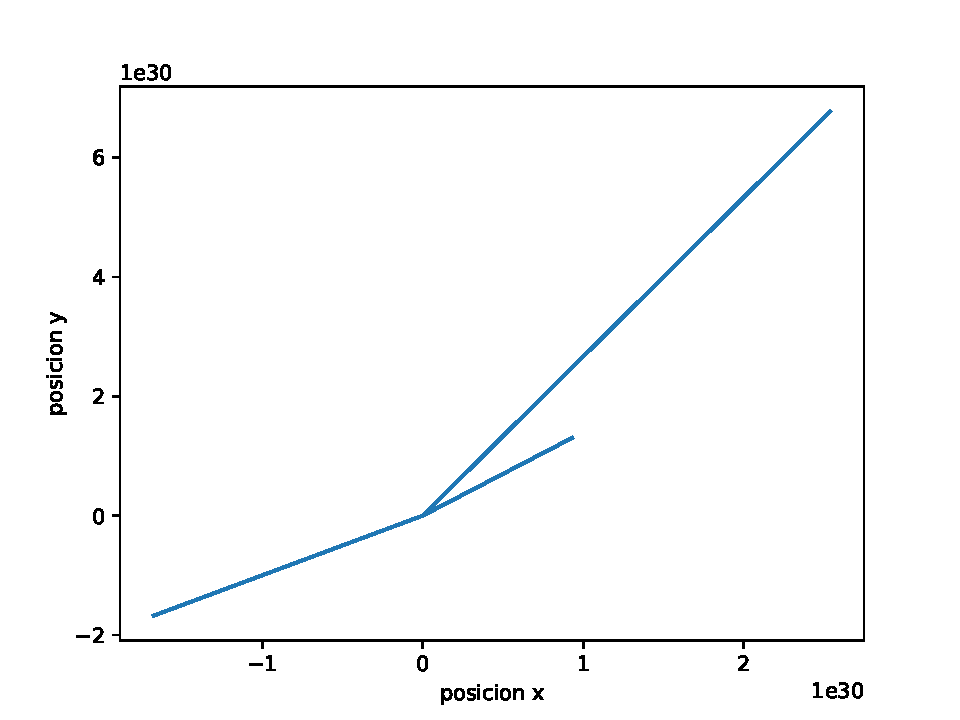
\includegraphics[width=0.75\textwidth]{grafsODE.pdf}

Deberia mostrar las diferentes trayectorias seg\'un el angulo de lanzamiento, pero por alg\'un error muestra lineas rectas

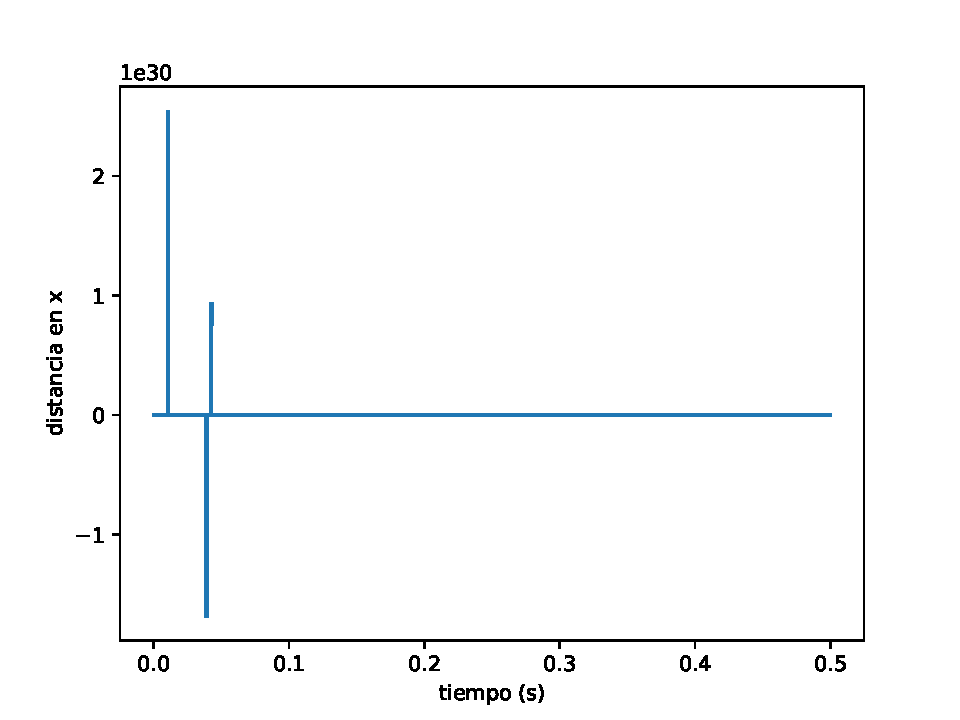
\includegraphics[width=0.75\textwidth]{grafsODE2.pdf}

Muestra la posicion en "x" con respecto al tiempo "t"
\end{centering}


\section{Ecuaciones diferenciales Parciales(PDE)}

\begin{centering}

\subsection{Fronteras fijas}
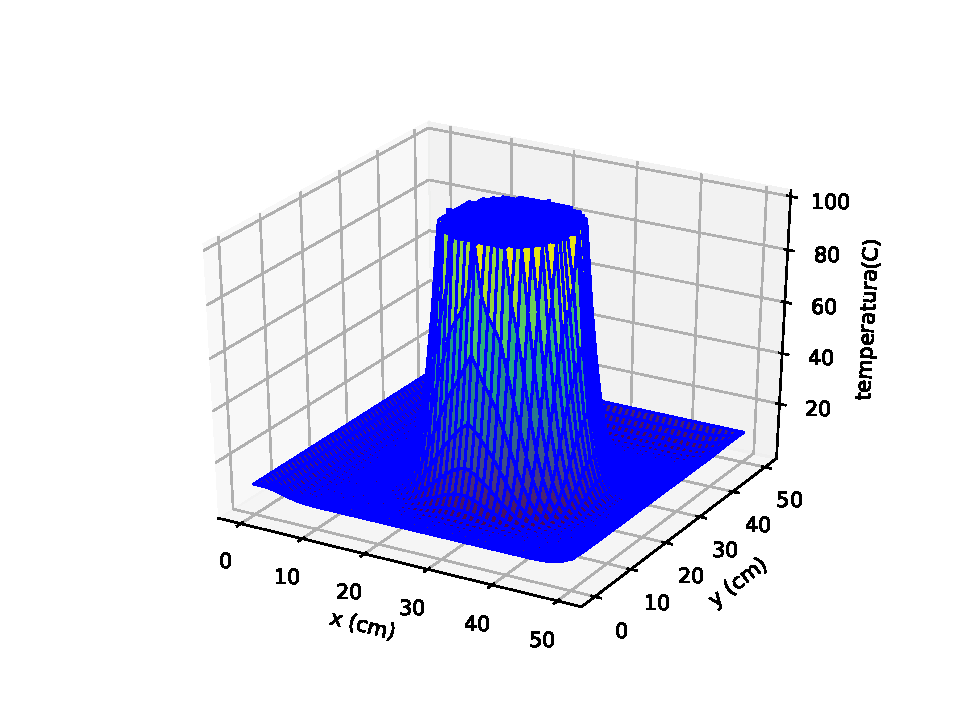
\includegraphics[width=0.75\textwidth]{3d2.pdf}
paso 10000
\\
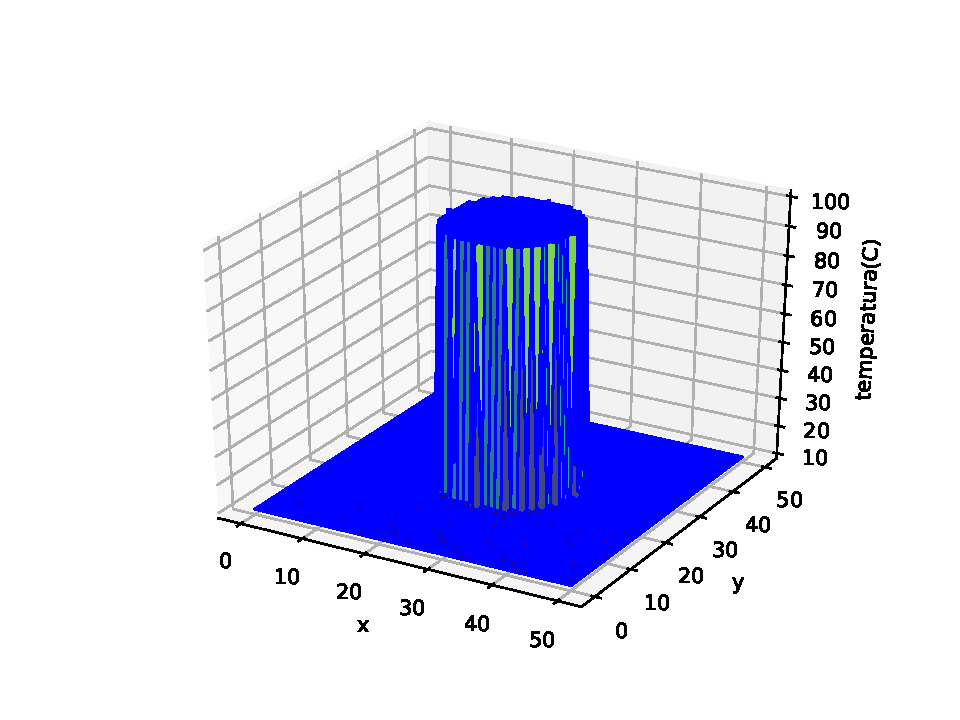
\includegraphics[width=0.75\textwidth]{3d3.pdf}
Paso 100
\\
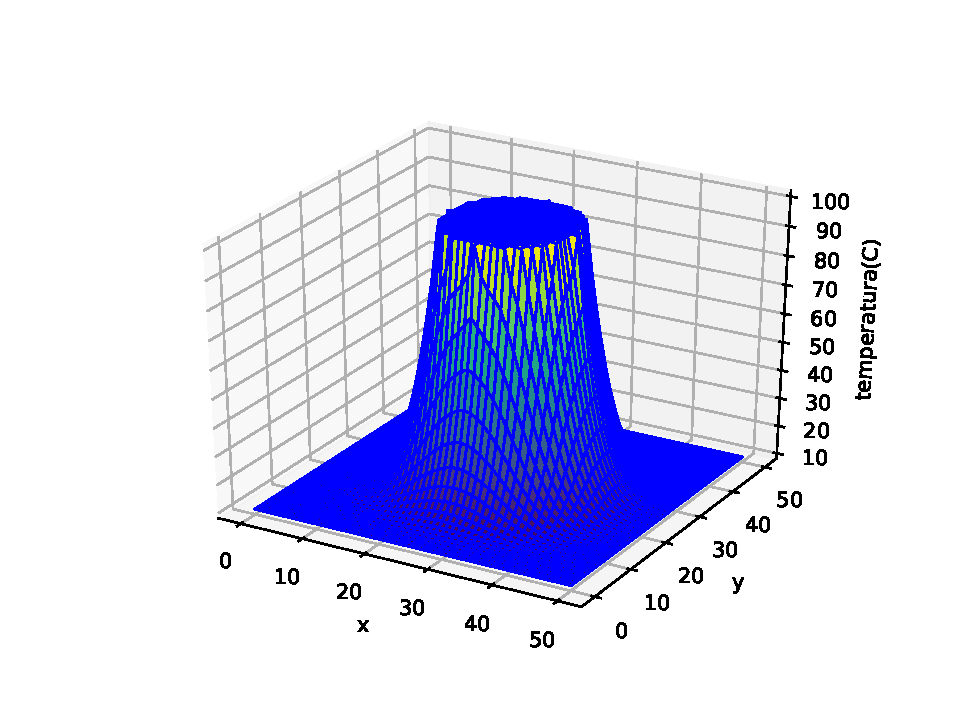
\includegraphics[width=0.75\textwidth]{3d4.pdf}
paso 1500
\subsection{fronteras abiertas}
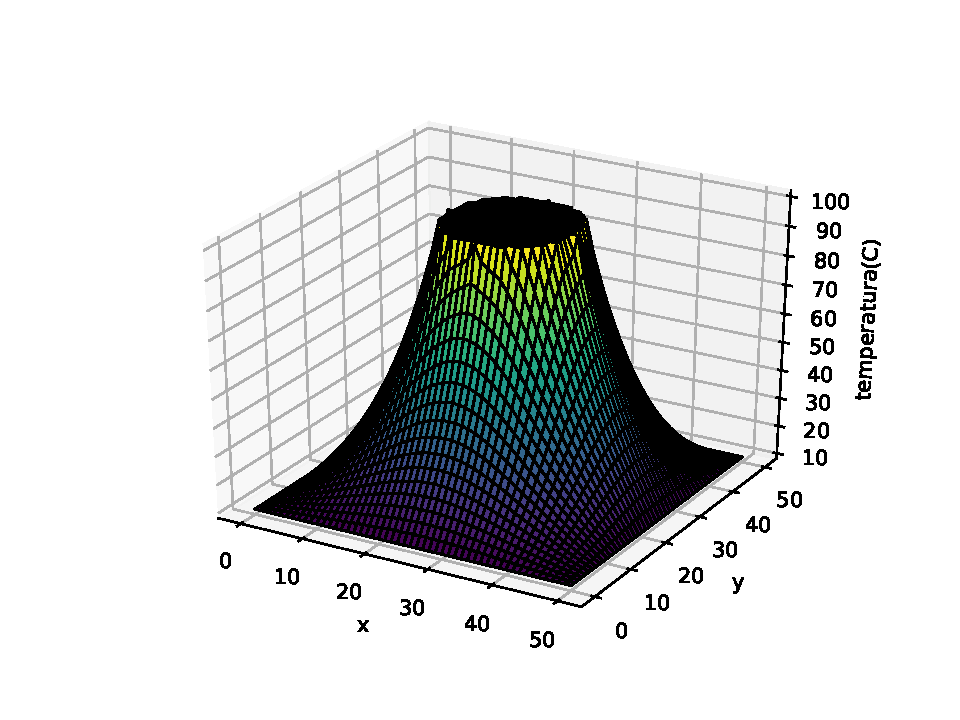
\includegraphics[width=0.75\textwidth]{3d5.pdf}
paso 10000
\\
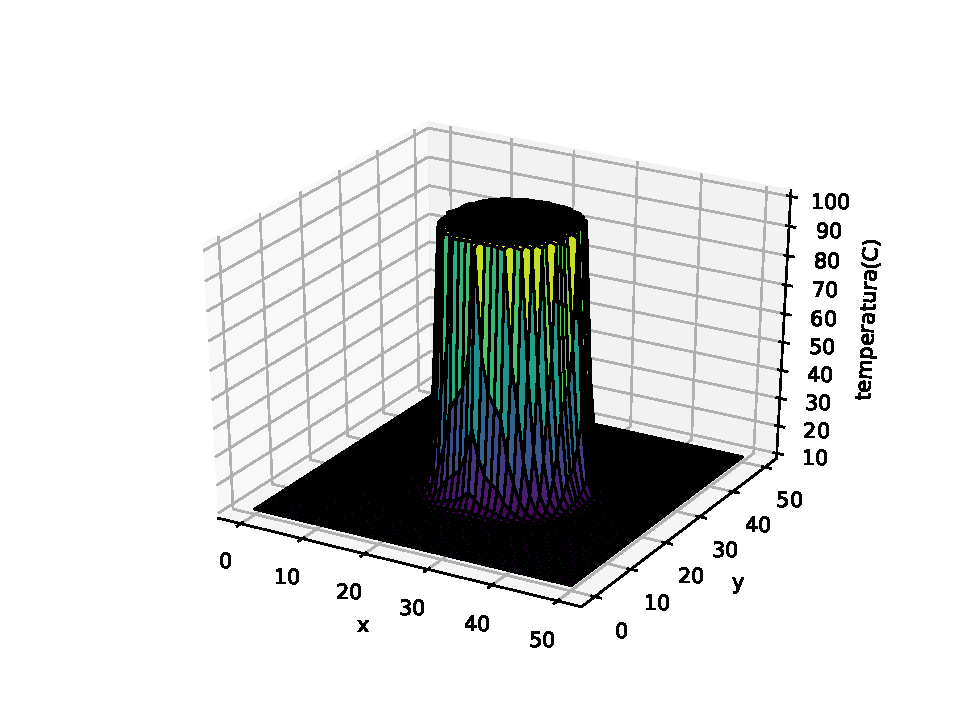
\includegraphics[width=0.75\textwidth]{3d6.pdf}
paso 100
\\
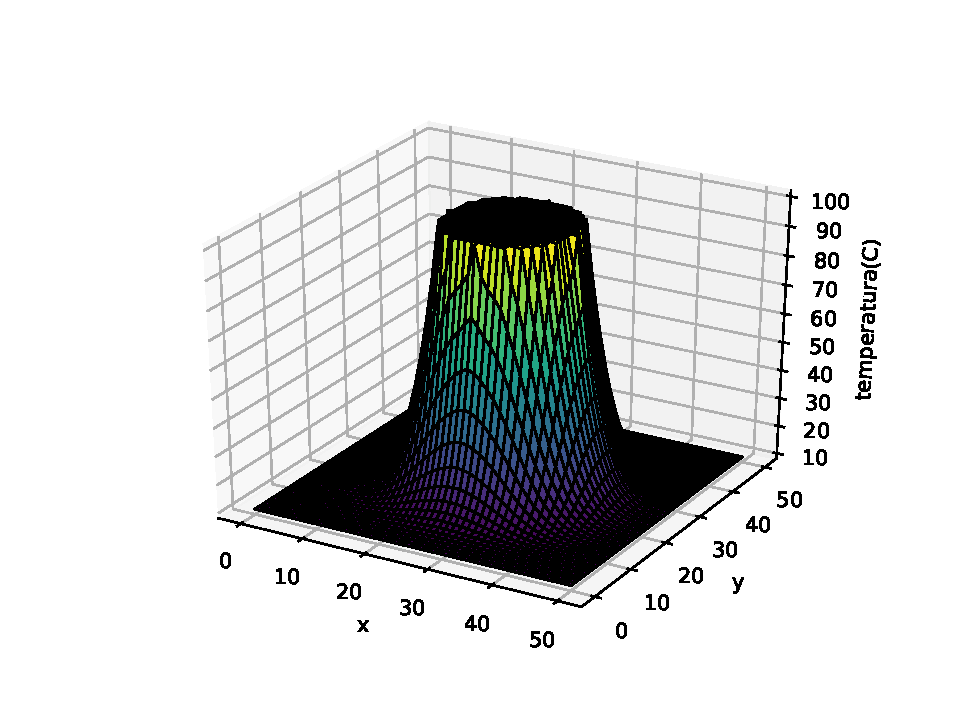
\includegraphics[width=0.75\textwidth]{3d7.pdf}
paso 1500
\subsection{fronteras periodicas}
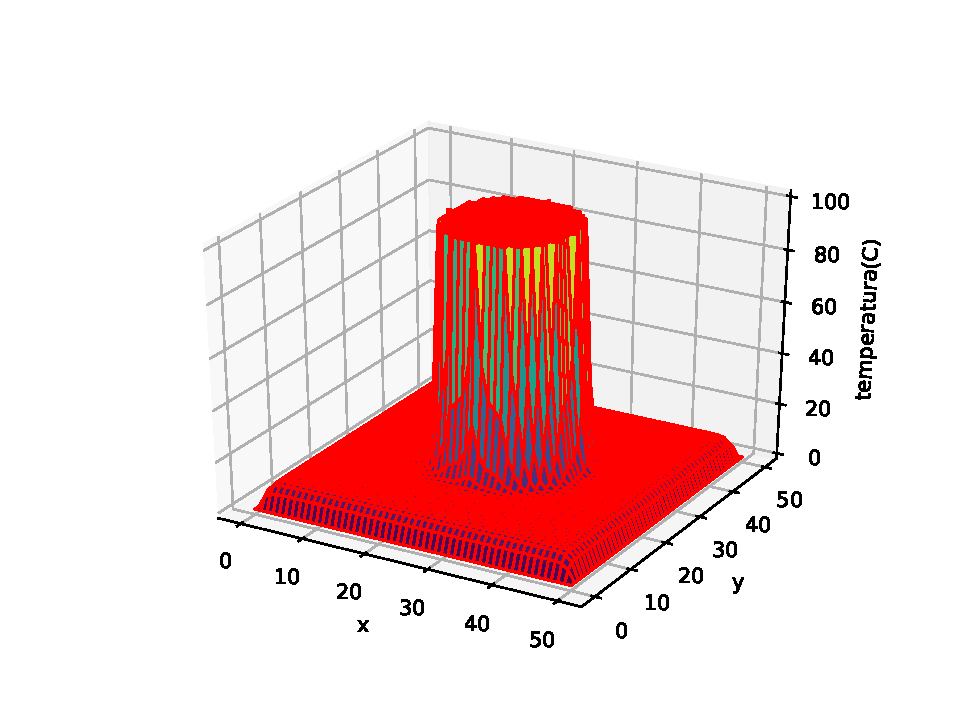
\includegraphics[width=0.75\textwidth]{3d8.pdf}
paso 10000
\\
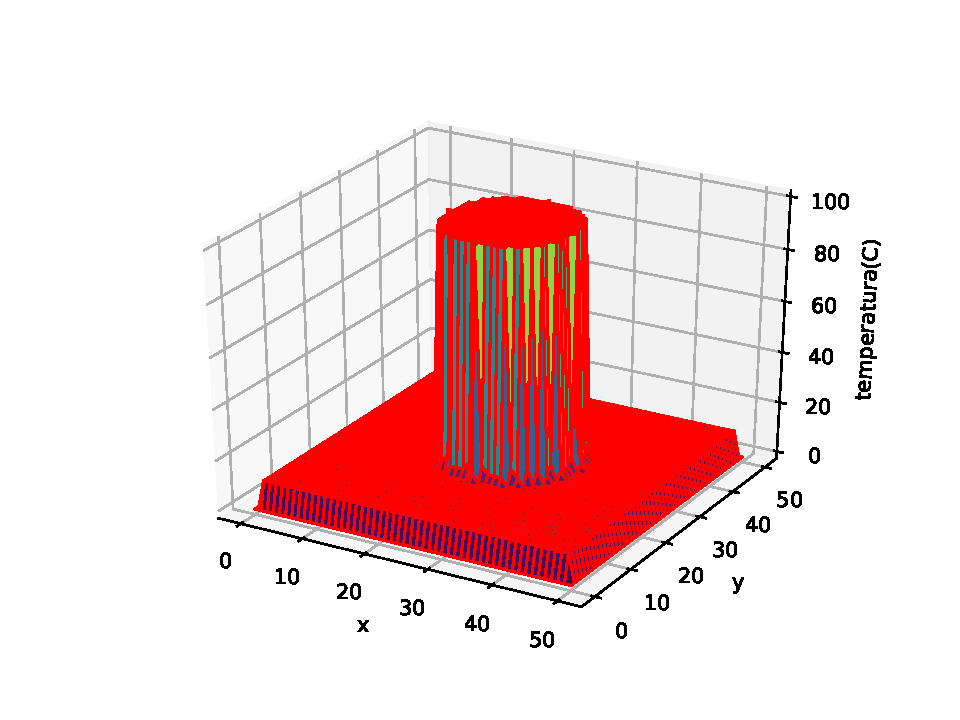
\includegraphics[width=0.75\textwidth]{3d9.pdf}
paso 100
\\
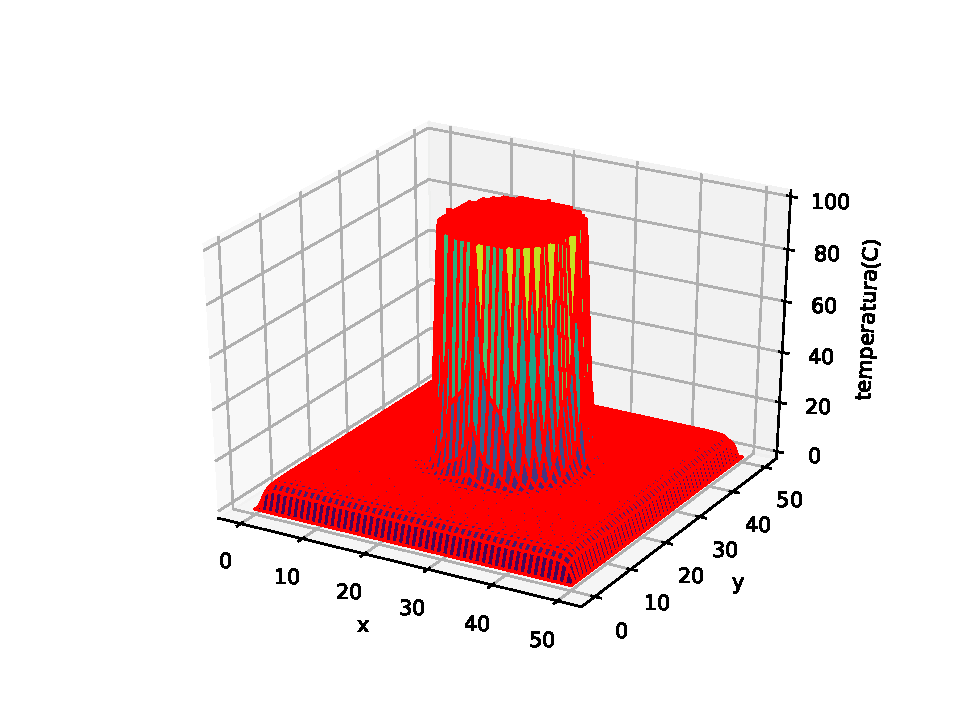
\includegraphics[width=0.75\textwidth]{3d10.pdf}
paso 1500


\end{centering}

 
\end{document}
